\documentclass[11pt,a4paper]{article}
% Compile with XeLaTeX (fontspec and xeCJK).
\usepackage{fontspec}
\setmainfont{LibertinusSerif}[Extension=.otf,UprightFont=*-Regular,BoldFont=*-Bold,ItalicFont=*-Italic,BoldItalicFont=*-BoldItalic]
\setsansfont{LibertinusSans}[Extension=.otf,UprightFont=*-Regular,BoldFont=*-Bold,ItalicFont=*-Italic]
\usepackage{xeCJK}
\setCJKmainfont{Hiragino Mincho ProN}
\xeCJKDeclareCharClass{Default}{"00B0, "00B7, "2013, "2014, "2018 -> "201F, "2026}
\usepackage[english]{babel}
\usepackage[a4paper,margin=2.5cm,top=2.3cm]{geometry}
\usepackage{graphicx}
\usepackage{xcolor}
\usepackage{titlesec}
\usepackage{fancyhdr}
\usepackage{enumitem}
\usepackage{xurl}
\usepackage[hidelinks]{hyperref}
\definecolor{accent}{RGB}{31,73,125}
\definecolor{muted}{RGB}{93,104,119}
\hypersetup{colorlinks=true,urlcolor=accent,linkcolor=accent,pdfauthor={Romain Fernex},pdftitle={Is an Asian NATO possible? The Quadrilateral Security Dialogue and the challenges of strategic cooperation in the Indo-Pacific}}
\urlstyle{same}
\setlist[itemize]{topsep=.25em,itemsep=.15em,parsep=0pt,leftmargin=1.4em}
\setcounter{secnumdepth}{0}
\titleformat{\section}{\large\bfseries\color{accent}}{}{0em}{}
\titlespacing*{\section}{0pt}{1.6em}{.6em}
\setlength{\parindent}{1.2em}
\setlength{\parskip}{0.35em}
\pagestyle{fancy}
\fancyhf{}
\fancyhead[L]{\small\color{muted}Romain Fernex}
\fancyhead[R]{\small\color{muted}\itshape Is an Asian NATO possible?}
\fancyfoot[C]{\small\color{muted}\thepage}
\renewcommand{\headrulewidth}{0pt}
\newcommand{\partbreak}{\par\begin{center}\color{muted}$\ast$\quad$\ast$\quad$\ast$\end{center}\par}


\begin{document}
\thispagestyle{empty}
\noindent{\small\sffamily\color{accent}\MakeUppercase{Indo-Pacific security}}\par\medskip
\noindent{\LARGE\bfseries Is an Asian NATO possible?\par}
\smallskip\noindent{\large\itshape The Quadrilateral Security Dialogue and the challenges of strategic cooperation in the Indo-Pacific\par}
\medskip
\noindent{\color{accent}\rule{\linewidth}{0.8pt}}\par\smallskip
\noindent{\small\color{muted}Romain Fernex · 2022 · Article in English}\par\bigskip

\begin{center}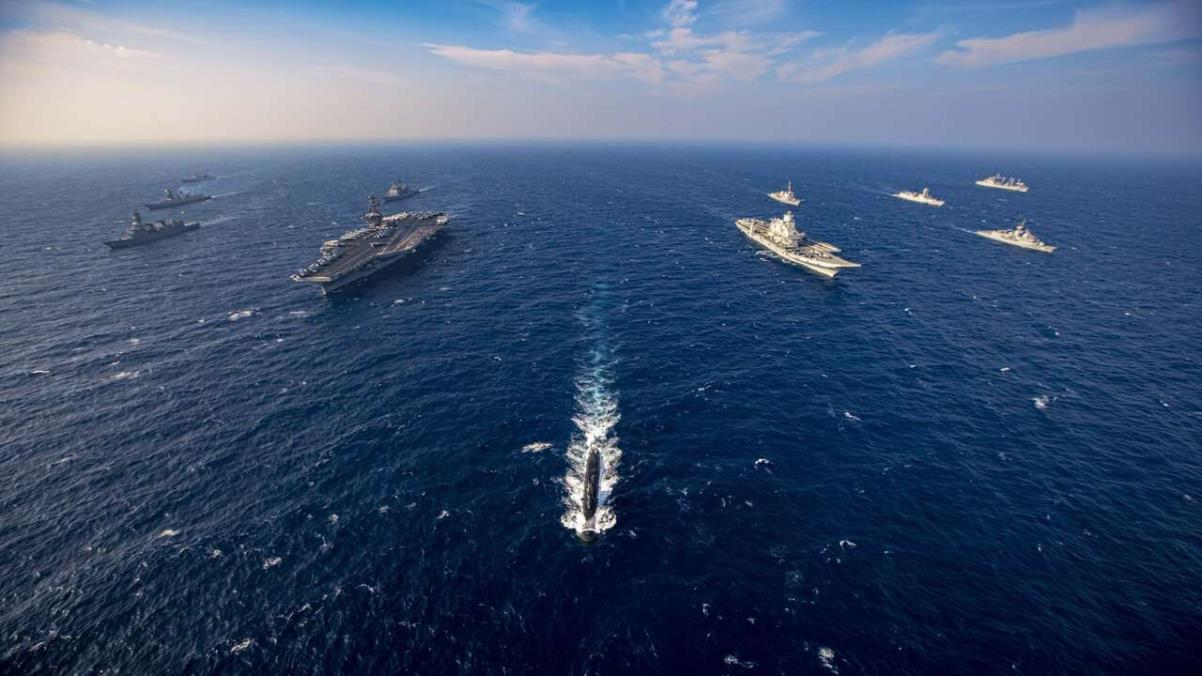
\includegraphics[width=\linewidth,height=6cm,keepaspectratio]{quad-cover.jpg}\end{center}

\section{Origins of the Quad}

On the 29\textsuperscript{th} of June, the first NATO summit attended by the organization’s partners in the Indo-Pacific area was held in Madrid. The Indo-Pacific region is a strategic area of vital importance for the United States, which defines it as stretching from the west coast of the United States to the Indian Ocean{[}1{]}. It accounts for more than two-thirds of the world’s economy and encompasses more than 50\% of the world’s population. Its importance is all the greater as tensions in Europe have accelerated the shift of the “centre of the world” towards this area, though this shift was already well underway since 1985. Thus, on the occasion of this summit, the Secretary General of NATO, Jens Stoltenberg, mentioned the challenge posed by the war in Ukraine and its destabilising effects, but he also took advantage of this opportunity to emphasise the increasingly worrying tensions in the South Pacific area. He underlined, in a more or less veiled manner, the risk posed to international security by the rise of China. While this position is not historically surprising, given that it largely echoes the strategic vision defended by the United States for several decades, the fact that it addresses this issue outside the traditional framework of bilateral and trilateral alliances that still dominate relations in the Asia-Pacific is not insignificant. Indeed, for the United States and its allies, the issue of China’s “containment” {[}2{]} is usually addressed through agreements such as the US-Japan Mutual Cooperation and Security Treaty adopted on 16 May 1960, which remains one of the pillars of the US presence in the Indo-Pacific. However, this does not mean that these countries should join NATO, as John Kirby{[}3{]}, Coordinator for Strategic Communications at the Security Council in the White House, pointed out. Therefore, one may wonder whether, in the absence of an extension of NATO, a similar alliance structure is still possible in Asia outside the strictly economic domain.

In this respect, some political analysts stress the importance of informal groupings that already exist and that could potentially, especially in the current geopolitical context, lead to the creation of real alliances whose role and nature would be similar to NATO. Among these groupings, one appears more promising than others, the Quadrilateral Security Dialogue (or Quad). This initiative launched in 2007 and revitalized in 2017, which brings together Japan, Australia, India and the United States, also made headlines recently with its fourth summit held on 24 May 2022 in Tokyo, just over a year after the previous summit in March 2021. The acceleration of the Quad has thus promptly come under criticism, particularly from China, which has described it as “a clique that could start a new Cold War”, in the words of Chinese Foreign Minister Wang Yi in March 2021. Yet the Quad in its current form has no military dimension and its security component remains relatively anecdotal due the differences of opinion between Quad members, notably between India and the US, on what the Quad should be aiming for.

Therefore, what is the Quad at present, what are the dynamics that drive its evolution, and which are facing each other, and is there any reason to see the Quad, as the PRC and some of its partners have called it, as a future Indo-Pacific NATO? These are the questions that this series of three separate articles will try to answer. The first one will deal specifically with the origins of the Quad and its current form. Then, another will try to describe the current position of Quad members and clarify why they may differ from one another. Finally, the last article will be aimed at questioning the feasibility and relevance of making the Quad the “NATO of Asia” by proposing and dissecting different scenarios for its evolution.

First of all, before looking at the creation of the Quad, it is important to emphasize that it is far from being the first multilateral initiative in the Indo Pacific. In the economic field, one can mention the ASEAN, founded on August 8 1967 by the Bangkok declaration, which already has about ten members. Besides, its regional forum which has been taking place every year since 1994, already gathers 27 countries, the majority of which are not ASEAN members{[}4{]}, such as Japan, South Korea, China, India and the United States. In the strategic area, which is the one this article focuses on, the SEATO, founded on September 8 1954 in the midst of the Cold War by the United States and joined by 7 other states, was intended to be a real Asian NATO. It was later dismantled on June 30 1977. But if SEATO disappeared with the warming of relations between Asian countries despite the Cold War, the ever-growing tensions in the region inevitably raise the question of the return of similar forms of cooperation.

The Quad did not, however, originally appear as a response to these new tensions: Indeed, the operational bases of the Quad were laid with the humanitarian aid campaign conducted jointly by the future members of the Quad during the boxing day tsunami that hit the coasts of the Asian Pacific countries in 2004. The goal was for these 4 countries to coordinate their efforts to provide help to disaster-stricken countries in the region. This is consistent with an important objective of the Quad, especially in its current form, which is to contribute to the development of the countries of the South Pacific by providing a multilateral alternative to the mainly bilateral aid offered by China. The ideological basis of the Quad is to be found in a speech, known as the “confluence of the two seas speech”, given by Shinzo Abe in 2006, when he was a candidate for the post of prime minister in Japan. During this speech, he called for the constitution of a “network of states united around the principle of freedom and around the rule of law (international law in this case) which would extend from one end of the Eurasian continent to the other”. This vision, also shared by the Japanese Foreign Minister at the time, Taro Aso, was supported by Indian Prime Minister Manmohan Singh and then by US Vice President Dick Cheney, which led to a first meeting of the members of the quad in May 2007 on the sidelines of the ASEAN forum in Manila. However, shortly after this meaningful step forward, the newly born Quad faced important challenges which led to its “dissolution” less than a year later. Indeed, China’s opposition to the project was a cause for concern for several members of the Quad which were still economically dependent on it, notably Australia, whose Prime Minister Kevin Rudd, elected in 2007, refused to attend the January 2008 Quad summit. South Korea, another strategic ally of the United States in the region, also voiced its skepticism regarding the Quad, which it considered too openly confrontational with China.

However, despite this failure, the members of the Quad continued to strengthen their cooperation through several bilateral and trilateral agreements: One example is the Communication, Compatibility and Security Agreement signed between India and the United States in 2015. As regards military initiatives, the Malabar exercises, launched in 1992 between India and the United States, saw the participation of Japan for the first time in 2015. Similarly, the air defense exercise of the Australian forces Pitch Black in 2019 took place in cooperation with the Indian army. These cooperative ventures all benefited from a favorable context with the escalation of tensions between China and India, which led to an armed confrontation between the two countries at the Doklam Tripoint along the LAC in the summer of 2017. Naturally, The return of Shinzo Abe to the position of Prime Minister of Japan in 2012 also played a key role in this widespread effort to bring former Quad members together. Thus the second Quad Summit took place, again in Manila, on November 12, 2017. On the agenda was the importance of denuclearizing North Korea, maintaining freedom of navigation in the Indo Pacific and the emergence of the “free and open Indo Pacific” concept that is central to the Quad’s objectives. This return of the Quad aroused, to no surprise, the ire of China and Russia, whose Foreign Minister Sergei Lavrov joined Wang Yi’s criticism of NATO and the Quad. The resolutely provocative stance towards China of the US Secretary of State Mike Pompeo under the Trump administration also contributed to give credence to Chinese claims of the Quad being “anti-China” among other states in the region outside the Quad.

Despite this, the Quad remains, nowadays, an informal grouping, focused on adherence to common values and still lacks any real military or institutional ambitions. This “democratic security diamond”, as described by former Japanese Prime Minister Shinzo Abe, which was intended to oppose the authoritarian powers on the rise in the region, seems paradoxically devoid of a security component. Fact is that the Quad 2021 joint statement, which specifies the main objectives and working groups set up within the framework of the Quad, mostly mentions groups dedicated to the vaccination effort in the face of Covid 2019, technology sharing etc... Though it also reaffirms the willingness of its members to guarantee a maritime order based on international law, it does not directly mention China as a threat to this order neither does it call for stepping up military efforts to contain it. However, this current state should not be considered immutable and the differences in perspective that exist between the members of this organization might lead to a total overhaul of the Quad depending on which one ends up dominating its development. This is what the next section will try to clarify by analyzing in detail the different realities faced by Quad members, what conceptions of the latter they defend and how their positions could possibly change in the face of the major crises of the last 5 years.

\textbf{Notes:}

\textbf{{[}1{]}} I am relying on the definition given in a White House memo on US Indo-Pacific strategy published in February 2022, which in many respects is similar to the definition of “Broader Asia” referred to by Shinzo Abe in his Confluence of the Two Seas speech. The document in question is the following: \url{https://www.whitehouse.gov/wp-content/uploads/2022/02/U.S.-Indo-Pacific-Strategy.pdf}

\textbf{{[}2{]}} The term used here is in quotation marks because it is used in a deliberately anachronistic way. It was originally coined by the American diplomat George F. Kennan in 1946, who used it to describe the strategy of the United States against the communist world during the Cold War. One goal of this article is, indeed, also to question the relevance of a bipolar vision of Indo-Pacific rivalries opposing a Sino-Russian bloc to a democratic bloc embodied by the Qaud. But this particular issue shall be dealt with in more details in the final section of this article.

\textbf{{[}3{]}} Full quote from John Kirby: “[...] And this isn’t about an Asian version of NATO. NATO is a transatlantic security alliance, the most effective, the most viable one in the world, the most successful one in the world.” It is taken from the following document: \url{https://www.whitehouse.gov/briefing-room/statements-releases/2022/06/23/press-briefing-by-press-secretary-karine-jean-pierre-and-national-security-council-coordinator-for-strategic-communications-john-kirby/}

\textbf{{[}4{]}} It should be noted that China, Japan and South Korea are members of ASEAN+3, an initiative to expand ASEAN led by Singapore, whose first meeting was held in 1997 at the Singapore Summit.

\section{The members’ perspectives}

The Quad’s members share principles, but what methods shall be used to achieve its objectives is the subject of significant debates between member countries who want to make it a real military and strategic alliance in the face of the rise of China and those who wish to maintain it in its current form and limit the risks of confrontation as much as possible. These are the trends the present article will analyse by considering the point of view of the various actors involved in this debate.

First, let’s look at the stance of the United States, the Quad’s main military power and unique in that it is relatively distant geographically from the other members. According to the White House memo {[}1{]}, the US has so far cautiously avoided mentioning the Quad in its plan to strengthen the security of the Indo-Pacific area. Indeed, it is only mentioned in the “building connections within and beyond the region” section of the report, which focuses on the Quad’s role in combating epidemiological risks, helping to develop infrastructure and promoting education through the new Quad Fellowship programme{[}2{]}. In comparison, the “Bolstering Indo-pacific security” section solely touched on the bilateral alliances forged by the United States with other States in the region and on the new trilateral alliance AUKUS announced on 15 September 2021 between the United States, Australia and the United Kingdom. However, the fact that this report opens with a quote from Joe Biden at the Quad summit, held only a few days after the AUKUS announcement, reflects the special place it occupies in the US vision of the indopacific. In fact, a survey conducted by the Center for Strategic \& International Studies (CSIS), an American think tank based in Washington DC, among representatives of the national elites of the Quad member countries and published in March 2020 shows that the United States is ready to support an institutionalization of the Quad and would not be opposed to a real military cooperation policy. Indeed, to the question “to what extent would you support the creation of a permanent Quad secretariat, with a presidency that rotates every three years among the members?” American respondents answered overwhelmingly positively. Responses were more mixed when asked about the creation of a standing armed force made up of the armies of Quad members, but the crisis in Ukraine is likely to tip the balance in favour of this proposal in the United States. This is even more likely as the struggle for influence between China and the United States in the region has long been theorised by US elites and keeps gaining credence among its “democratic bloc” allies. To quote Richard Hass, President of the Council on Foreign Relations (CFR) in the magazine Foreign Affairs in 2021: “the rise of authoritarian states challenges the power and leadership of the US”. This goes to show that, as the competition between the PRC and the US is intensifying, American elites are more and more outspoken about pushing for a strong containement policy towards China. A competition that also prompts other indopacific states to enter the fray, as Yan Xuetong, researcher at Tsinghua University in Beijing, pointed out in the Chinese Journal of International Politics in 2020, asserting that “the Sino-American competition creates pressure on the other regional powers [forcing them] to take sides either with the United States or with China”. However, this aspiration to create a real democratic bloc in the Asia-Pacific must be qualified: Indeed, although China has been critical of a potential “Asian NATO”... in the run-up to the NATO forum in Madrid in June 2022, Jens Stoltenberg, NATO Secretary General, dismissed these accusations with a rhetorical question insisting that such a project was never on the agenda. Yet while the United States still has many bilateral and trilateral alliances in the region, the need for a full-fledged military alliance may potentially arise in the near future.

Now regarding Japan: As the country that initiated the Quad, it attaches particular importance to it and, according to the survey mentioned above, is also in favour of institutionalising it. However, it has never mentioned making it a military alliance, and while its position on this subject is certainly less clear-cut than in the case of India, the Japanese elites seemed to rule out such a development at the time of the survey. However, there is an important commonality between the Japanese position and the US position, which is the idea of establishing a united front against China. Indeed, at the Quad summit in Tokyo in May 2022, Japanese Foreign Minister Hayashi Yoshimasa supported the increasingly assertive US position on Taiwan. This earned him a warning from his Chinese counterpart, followed by a Sino-Russian show of force with the deployment of 6 strategic bombers that flew over Japanese territory. These worries about an increasingly troublesome Chinese neighbour also punctuated Joe Biden’s visit to Tokyo in May this year, as highlighted by Jean Yves Colin, member of the board of directors of the French think tank Asia Center and expert on North Asia. Apart from Taiwan, Jean Yves Colin put the emphasis on more pressing issues for Japan notably its “territorial security concerns” over the Senkaku Islands and the Yonaguni Island. Thus, in this very tense context, Japan intends for the Quad to play a major role in ensuring States sovereignty on their territory, both on land and at sea. Fact is, at the May 2022 Quad Summit, the Japanese Prime Minister Fumio Kishida did not hesitate to, in the words of Jean Yves Colin, “draw a parallel between the situation in Ukraine and the Indo-Pacific”{[}3{]}. This position thus seems consistent with the concept of the “democratic security diamond” enunciated by Shinzo Abe in 2006 and reflects the vision of a strong group capable of imposing these values in the Indo-Pacific space. Yet it remains vague regarding the nature of the means to be used to achieve this objective. In fact, most of the military cooperation campaign undertaken by Japan is carried out in the framework of its alliance with the United States, and vice versa. For example, the National Security Strategy report published by the US Department of Defense in 2013 explicitly states that “the US-Japan Security Treaty is the cornerstone of Japan’s security”. A strategic partnership that the two states have sought to develop with, for example, the Legislation for Peace and Security in 2015. It should also be noted that Japan does not only see its own security through this alliance but also that of its interests in the entire Indo-Pacific area. Shinzo Abe has indeed called the EU-Japan Security Treaty an “indestructible and immovable pillar” that helps “preserve peace in Asia, the Indo- Pacific and the world”{[}4{]}. However, Japan is also seeking to diversify its partnerships in Asia, including India, as demonstrated by its participation in the Malabar exercises in 2017. Therefore, forging a broader, multilateral alliance could help it in the pursuit of this goal.

Australia, on the other hand, has always been very critical of a militarised Quad, and particularly of a Quad that would overtly oppose China. This is largely due to its strong economic ties with the latter. Indeed, in 2020, China was the country’s main trading partner, far ahead of Japan and the United States, which greatly undermines its independence when it comes to thinking about the Quad. Australia also played a significant role in the failure of the Quad in the early 2000s by withdrawing from it in 2008 under the Kevin Rudd government. Nevertheless, of all the members of the Quad, the Australian position towards the Quad is probably the one that has evolved the most, even after its return in 2017: As the National Institute for Defense Studies (NIDS), a Japanese think tank, points out, Australia, which has always thought of Oceania as the main area for the exercise of its military and economic power, has had to face increasing competition from China in this same area and has engaged in a struggle for influence with the PRC. Fact is that the Covid 19 crisis, and more particularly the aid provided to the Pacific islands by these two countries, has fueled tensions between the two States. On the one hand, Australia has increased initiatives in cooperation with the World Health Organisation (WHO) and the World Food Program (WFP), adopting a decidedly multilateral model, while, China, on the other hand, has signed many bilateral aid agreements with countries that serve its interests. This major difference in approach has prompted the Australian government to take a much more hostile stance towards China than under Kevin Rudd. In April 2020, Australian Foreign Minister Marise Payne angered the PRC by demanding greater transparency about the origin of the SARS COV-2 virus and calling for an international enquiry into the issue on Chinese territory. The PRC retaliated by imposing higher taxes on barley imported from Australia and warned Chinese students, the largest international student population in Australia with almost 28\% of the international student body, that they could face discrimination while studying in Australia.

All of this took place in a tense political atmosphere within the Australian government itself with the revelation of corruption cases involving several politicians under the Rudd administration and the Chinese Communist Party in 2018. This led to the implementation of a law against foreign interference that same year and has pushed Australia to think about its evolution without China (if not against it for some government officials). It has also joined the Malabar 2020 exercises and strengthened its economic cooperation with the other members of the Quad, notably through expressing its desire to join the new Indo-Pacific Economic Forum (IPEF) project, which will bring together ten or so countries in this area {[}5{]}. Troy Lee Brown, a researcher in regional and maritime security at the University of Western Australia, said that Australia’s goal now would be “to offer an alternative to OBOR” in order to further reduce its attachment to China. Thus, in the CSIS survey, Australia emerged, along with the US and Japan, as one of the driving forces behind the strengthening of the Quad. This change was also accompanied by a change in tone in the Australian press. While the latter was initially critical of a strong Quad, some institutes, including the Australian Strategic Policy Institute (ASPI), are now questioning India’s cautious position, which it describes as the Quad’s “weak link”. It explains this by its important land border with China, which makes it strategically fragile, and stresses that it is the only member of the Quad without any concrete guarantee of security from the other members. Thus, he considers Delhi’s attitude to be more trilateral and asserts that it sees the Quad as a mere display case rather than a major project in the face of Chinese hegemonic ambitions. This oddly echoes Australia’s position during the Rudd government from the perspective of Japan and the US.

But what about India’s position according to Indians? The opinion of Indian elites gathered by the CSIS shows that this country is by far the most hostile to an institutionalisation of the Quad and to its overhaul into a strategic alliance. There are several reasons for this, some of which have already been raised by the Australian Strategic Policy Institute: firstly, India suffers from a major economic dependence on China and Russia, its close partner. An economic dependence that is also reflected at the military level with the massive purchase of Russian and Chinese equipment by the Indian army, although its main partners on the operational level are the United States and Japan with, among other things, the Malabar exercises. At the same time, India is very insistent on avoiding confrontation with China because it is already under heavy pressure from the latter. Conflicts over the Line of Actual Control (LAC) have been growing in intensity since the early 2000s and played a major role in the reintegration of India into the Quad in 2017 as discussed in the previous article. This direct threat to its territorial sovereignty is one of the main elements that distinguishes India from Australia and prevents it from making a strategic pivot as significant as that made by the latter. Thus, at the 4th India-US Summit in New Delhi in October 2020, the US Deputy Secretary of State, Stephen E. Biegun, made a speech echoing this very particular situation of India. He praised India’s tradition of ‘strategic autonomy’ and, while he shared his vision of a ‘Pax Indo Pacifica’{[}6{]} to protect the prosperity of the Indo-Pacific region, he also insisted that the security partnership between India and the United States did not have to involve the presence of US troops in the country. Similarly, although the importance of giving India the means to defend its sovereignty was central to his speech...the Quad was never mentioned as a tool of this security policy. This idea can be also be found in a statement by the Indian Army Chief General M.M. Naravane in the Economic Times in March 2021 who insisted that “there will definitely be bilateral military cooperation”, but that “the Quad is not a military alliance”.

Does this mean that India only envisions its defense policy through its bilateral alliance with the United States and does not have any major project for the Indo-Pacific region in response to China? Clearly, India has shown a real voluntarism on several occasions, including in the way it thinks and structures its opposition to China. On the military front, its efforts to increase military exercises with other Quad members and work on interoperability have undeniably played a significant role in the Quad’s progress since 2017. On the economic front, the Indo-Japanese Africa Asia Growth Corridor (AAGC) project launched by Indian Prime Minister Narendra Modi in May 2017 aims to offer an alternative to the One Belt One Road initiative (OBOR). Finally, India was the first member of the Quad to denounce the “One China policy” led by Beijing in 2010 by demanding the recognition of India’s sovereignty over Kashmir.

In short, India is forced to adopt an ambiguous position due to its dependence on China, but it is also the country most sensitive to China’s outbursts as they directly threaten its territorial integrity. Thus, the more significant it deems this threat to be, the greater the chances of a change of tone similar to that of Australia, although it remains to be seen exactly how this will be achieved and whether or not it will place the quad at the centre of this change.

To sum up, this article gave a little more detail the situation of the different parties involved and explained how they see the future of the Quad as well as how they perceive their own role in the Indo-Pacific area. Yet, the question of a possible extension of the Quad has yet to be answered. Therefore the next section, which shall conclude this series, will focus on outlining different possible scenarios for the Quad, including that of a ‘Quad Bloc’ with a role close to that of NAT, and will discuss the probability and, above all, the legitimacy of each of these scenarios in order to better understand their potential.

\textbf{Notes:}

\textbf{{[}1{]}} The note in question: \url{https://www.whitehouse.gov/wp-content/uploads/2022/02/U.S.-Indo-Pacific-Strategy.pdf}

\textbf{{[}2{]}} Program launched on September 24, 2021 by U.S. President Joe Biden, together with representatives of the other Quad members, allowing students from Quad countries (except the United States) studying for a master’s degree or doctorate in the best American universities in the field of science, engineering, mathematics and technology (STEM) to benefit from a Quad sponsored scholarship.

\textbf{{[}3{]}} The full quote given by Jean Yves Colin in his article is: “Russian aggression in Ukraine is a direct threat to the principles of the United Nations. We must not let the same situation happen in the Indo-Pacific.”

\textbf{{[}4{]}} Quote from a speech given by Shinzo Abele on 19 January 2020 on the occasion of the 60th anniversary of the signing of the Japan-U.S. Security Treaty. The full speech can be found in a press release from the Japanese Prime Minister’s Office via the following link: \url{https://japan.kantei.go.jp/98_abe/statement/202001/_00002.html}

\textbf{{[}5{]}} It is interesting to note that while China will not be part of this initiative, Taiwan will not join either, which shows that there is a willingness not to risk confrontation with the PRC. This more open stance prompts countries usually reluctant to openly oppose China, such as South Korea – a particular case to which we will return in detail in the next section – to join this initiative.

\textbf{{[}6{]}} The full quote from Stephen E. Biegun is: “One might call this a vision of a Pax Indo-Pacifica, a region at peace, protected and made prosperous in equal measure by those who comprise the Indo-Pacific.” The speech from which it is taken can be found here: \url{https://2017-2021.state.gov/remarks-by-deputy-secretary-stephen-e-biegun/index.html}

\section{Possible futures for the Quad}

Having considered the perspectives of the Quad’s members, it is now appropriate to consider what the Quad could potentially become in the future and the role it could play in the Indo-Pacific and elsewhere. In the light of our previous analyses, two very distinct scenarios seem to stand out: firstly, the evolution towards a “Quad Bloc”, militarised and, especially, institutionalised in response to a bloc formed by China and Russia. Then its opposite, with the continuation of a “withdrawn Quad” that refuses to display any strategic ambition and remains strictly confined to its role as a display case for Western democracies. Finally, this article will introduce a third scenario, whose strategic dimension would certainly be mostly economic, but which would benefit from real prerogatives to impose itself in the Indo-Pacific and propose a concrete alternative to the development model promoted by China.

First of all, what would a “Quad Bloc” look like? The term Bloc refers explicitly to Cold War logics and is therefore in line with the comments made by the PRC. This implies a Quad that would formally state its objective to stand against China and would present itself as a real alliance, though more limited in size than NATO, because it is based on a smaller but more tightly knit group of countries. But to analyse this scenario in more detail, we will start with an article by John Hemmings, professor at the Daniel K. Inouye Asia Pacific Center for Security Studies, published in the Journal of Indo-Pacific Affairs in April 2022, in which he argues in favour of a transformation of the Quad into a real military alliance. Here, John Hemmings uses a particular definition of the term “alliance”, which is that of Glenn Snyder {[}1{]} in Alliance Politics, who describes an alliance as “a formal association of states for the use of military force, in specified circumstances and against non-member states”. An alliance implies a form of commitment on members’ sides and creates an obligation for them to respect the terms of the treaty or secret agreement, or not, that led to its formation. A good example of this type of political entity would be the alliance between the US and Japan or between the US and Australia. According to Hemmings, it is this type of alliance that would be required to respond to the return of an increasingly ambitious China that worries the Western bloc. Thus, drawing on the neo-realist theses of Kenneth N. Waltz {[}2{]}, the author argues that democracies have an unfortunate tendency not to respond strongly enough to counter the influence of powers with clear hegemonic pretensions. He draws a parallel between the Triple Entente of 1914 and the Quad, pointing out that both are non-binding, and asserts that the Triple Entente failed to respond to the challenge of the German advance to a sufficient extent because of this hesitancy on the part of the democracies. Indeed, there is growing evidence of China’s ambition, as noted in several strategic reports issued by the governments of the Quad members. For example, in 2018, the US National Defense Strategy report spoke of a PRC that “continues its military modernisation programme and seeks to achieve regional hegemony in the Indo-Pacific”. The Defense White Paper published by the Japanese Ministry of Defence in 2021 and the Defense Strategic Update published by its Australian counterpart a year earlier made similar observations. For his part, Xi Jinping has repeatedly urged China’s People’s Liberation Army (PLA) – in March 2021, January 2021 and May 2020 – to be prepared for war at any time.

The development of a Sino-Russian bloc is also an important factor in the complex equation of Indo-Pacific military cooperation. For Andrew Yeo, Senior Fellow and SK-Korea Foundation Chair in Korean Studies at Brookings, NATO’s invitation to the Indo-Pacific countries is part of this logic and he believes that it “reflects an awareness of a deeper link between trans-Pacific security [...] due to increased cooperation between China and Russia”. A rapprochement that has been taking place for many years on the economic as well as military level with, for example, China’s participation in the annual Russian military exercise since 2018. It is accompanied by a process of distancing itself from the Western bloc, which keeps accelerating and is now reaching new heights with the war in Ukraine {[}3{]}.

Despite this, there are also strong counterarguments to this view: First, the viability of a real Sino-Russian alliance is far from clear. While Russia has no choice but to turn to China at the moment, it is in a particularly complex position, being unable to negotiate on an equal footing with the Chinese giant. Jae Seung Lee, professor and Jean Monnet Chair at Korea University, indeed pointed out, durin a conference held in Paris at Maison Suger, that it would be particularly complicated for Russia to assert its point of view in a world dominated by China and that its fragile position risks being rapidly exploited by the latter. Therefore, even if it seems impossible for the moment, if Russia wants to regain its independence and influence in the world it will have to find new partners, including in the Indo-Pacific area. Secondly, as explained in the previous article, the prospect of a “Quad Bloc” is very far from being unanimously accepted among Quad members, if not purely and simply unthinkable at the moment. Unless a major event occurs that causes its more reluctant members to reassess the threat presented by China and to decide to respond militarily, it is highly unlikely that a militarisation of the Quad will take place in the coming decade. Even if the crisis in Ukraine has been a catalyst for remilitarisation in Europe and the indopacific, there is little chance that it will be enough to push states to extend their ambitions beyond the bilateral or trilateral level. Finally, making the Quad a major player in the unification of the Indo-Pacific democratic bloc would be especially intricate in this scenario. Many countries in the Asia-Pacific area are still very dependent on China economically and will inevitably be much more reluctant to join an alliance that is openly in conflict with China. This could also pose other strategic challenges with significant repercussions even beyond the Indo-Pacific. In this respect, the case of South Korea is particularly interesting. At the same conference, Dr. Jae Seung Lee insisted that South Korea would most likely never seek to join a confrontational alliance with China for several reasons: The first, mainly economic, is related to supply chain issues as China produces the overwhelming majority of rare earths needed for the production of semiconductors and other high-tech products in which South Korea excels. The second, geopolitical, is that in order to negotiate with an increasingly restless North Korea, with a steadily advancing nuclear programme {[}4{]}, it is necessary to maintain good relations with China on which the DPRK is completely dependent. The denuclearisation of North Korea which was mentioned at this year’s Quad summit in Tokyo, therefore seems unfeasible in the case of a “Quad Bloc”, let alone the reunification of Korea. In short, such a development seems very unlikely at present. Conversely, it is likely that it will not find any real justification in the years to come, barring exceptional events.

Does this mean that a “withdrawn Quad” as mentioned in the introduction would be preferable? Opting for the exact opposite of the “Quad Bloc” would undeniably be a step backwards for the Quad, or at least a form of continuity with what it currently is. In its current state, its prerogatives are limited to say the least, if not non-existent, given that it is an informal group and not a full-fledged institution. This greatly restrains its field of action and if, in the economic field, it has already set up several aid programmes, which are already in effect, these initiatives still pale in comparison with those of associations such as the ASEAN. This is even more true in the military field, where almost all progress is made at the bilateral or trilateral level, which gives the impression that the influence of the Quad is only that of its most powerful member and therefore does not bring any real added value. On 3 June 2022, the Quad launched the Indo-Pacific Partnership for Maritime Domain Awareness (IPMDA), which comprises the deployment of satellites and other surveillance systems to combat illegal fishing – which China has made a specialty of, especially in the East and South China Seas – as well as the sharing of information with partner countries such as Singapore and the Solomon Islands. An apparently ambitious initiative that China, through the intermediary of its foreign minister, did not fail to criticise, arguing that the aim of the Quad with the IPMDA was to “contain China” and “make other Asia-Pacific countries pawns of American hegemony”. However, this remains an essentially preventive measure and the capacity of the states involved in this effort to concretely fight against repeated incursions into their EEZ has yet to be proven. Therefore, while this type of Quad would undoubtedly draw more candidates to participate in its expansion, it would mainly play the role of a showcase for democracies rather than that of an actor capable of imposing itself in the Indo-Pacific. It would therefore be incapable of responding to the major challenges facing the region and would undoubtedly lose most of its interest.

Nonetheless, one may now wonder whether there is an alternative path to these two extremes? Certainly, making the Quad a true military alliance seems complicated and undesirable, but an institutionalized Quad would still have a genuine potential in terms of economic strategy. On the condition that the number of member states is limited, it could allow for a much stronger economic integration of the main powers active in the Indopacific area and help them detach themselves, at least partly, from their economic dependence on China. Such a development would be far from useless on the geopolitical level by giving a broader wiggle room to countries such as India to rethink their positioning, including on the military level. Similarly, an ambitious economic and technological integration effort on the part of the Quad could provide the necessary impetus for other forms of economic cooperation currently in development, such as the IPEF or the AAGC, to compete with the PRC’s “One Belt One Road” initiative. To return to South Korea, if a more frontal opposition to China could discourage it from joining a “Quad +”, it could also enable it to face its supply chain problems more serenely. According to CSIS, being part of the Quad would also enable it to assert more strongly its positions on the regional and international scene, including regarding North Korea, with the support of the United States. However, the CSIS also acknowledges that this integration is necessarily conditional on the guarantee of an unwavering support from the latter, given the risks that a Chinese reaction could entail. While China will not necessarily opt for a concrete economic or military response, if this were to happen it is imperative for Korea and any other country aspiring to join the Quad to have the protection of Washington and of the other members of the Quad. If the Trump administration and its many foreign policy inconsistencies have permanently eroded the trust placed in the US by its allies, including South Korea, Biden’s promotion of a “free, open and rules-based Indopacific” seems more in line with this need. However, as the French newspaper Le Monde underlined in an article published on 29 June 2022, “the importance of the Quad for Biden is still difficult to determine” and the value he will place on it in the face of other competing projects such as the AUKUS partnership needs to be clarified in order to be able to think about the future of the Quad.

In conclusion, the shape the Quad will take in the future depends on many factors outside the control of states, but it is their personal stance that will ultimately determine the direction of its evolution. Without clear support and genuine leadership from the United States, it is unlikely to become institutionalised, let alone a significant player in the Indo- Pacific geopolitical order. Similarly, if India and the countries likely to join the Quad do not see the threat posed by China as outweighing the benefits of preserving their economic interest with China, it is radically impossible for the Quad to grow much larger than it is at present. That is to say the likelihood of an Asian Nato based on the Quad is indeed low, but, should Asia Pacific countries be willing to place their faith in a stronger, well organized Quad, they might very much benefit from it.

\textbf{Notes:}

\textbf{{[}1{]}} The original quote by Glenn Snyder, Professor Emeritus of Political Science at the University of South Carolina, to define what an alliance is, is the following: “formal associations of states for the use of military force, in specified circumstance against states outside their own membership”

\textbf{{[}2{]}} The concept of neo-realism in geopolitics was developed by Kenneth N. Waltz, one of the most renowned political scientists in the field of international relations and a faculty member at UC Berkeley and Columbia, in his 1979 book \emph{Theory of international politics}. This theory leaves little room for cooperation in international relations and emphasises competition and conflict as major components of the geopolitical order.

\textbf{{[}3{]}} It is interesting to note that already in 2021, during a visit to China by the Russian Foreign Minister, Sergei Lavrov, he expressed the importance of exiting the SWIFT system by stressing his desire to “bolster technological independence and move away from international west controlled payment system”.

\textbf{{[}4{]}} Among the major advances made by North Korea in recent years in the field of military nuclear power, we can cite the development of the Hwasong-12 IRBM (intermediate-range ballistic missile) in January 2021, capable of hitting Alaska, or, more recently, the Hwasong- 15 ICBM (intercontinental ballistic missile) which could potentially hit the United States’ mainland.

\section{Sources}

\begin{itemize}
  \item \textbf{Japanese Press}
  \begin{itemize}
    \item \url{https://english.kyodonews.net/news/2022/06/1345330ff0f8-no-asian-nato-says-us-as-alliance-brings-japan-s-korea-to-summit.html}
    \item \url{https://www.japantimes.co.jp/news/2022/06/20/national/japan-korea-australia-new-zealand-nato-meeting/}
    \item \url{https://www.japantimes.co.jp/news/2022/06/29/national/japan-sk-us-talks/}
    \item \url{https://asia.nikkei.com/Politics/International-relations/Japan-will-turn-to-Quad-in-new-Cold-War-Defense-Ministry-think-tank}
  \end{itemize}
  \item \textbf{British Press}
  \begin{itemize}
    \item \url{https://www.bbc.com/news/world-asia-india-61547082}
  \end{itemize}
  \item \textbf{North American Press}
  \begin{itemize}
    \item \url{https://thediplomat.com/2017/11/why-has-australia-shifted-back-to-the-quad/}
    \item \url{https://foreignpolicy.com/2020/10/08/why-quad-alliance-trump-cares-about-india-australia-japan-china/}
    \item \url{https://www.voanews.com/a/japan-s-kishida-considers-joining-nato-summit--sources/6603976.html}
    \item \url{https://www.voanews.com/a/what-to-expect-from-south-korea-s-first-nato-summit/6635935.html}
    \item \url{https://edition.cnn.com/2021/03/11/asia/quad-us-india-japan-australia-intl-hnk/index.html}
    \item \url{https://time.com/6188414/japan-south-korea-nato-summit/}
  \end{itemize}
  \item \textbf{Australian Press}
  \begin{itemize}
    \item \url{https://www.aspistrategist.org.au/india-and-the-quad-weak-link-or-keystone/}
    \item \url{https://www.news.com.au/technology/innovation/the-quad-launches-bold-plan-to-combat-chinas-dark-ships/news-story/4aedcc8c4403199b8bd5ab69c410305a}
  \end{itemize}
  \item \textbf{French Press}
  \begin{itemize}
    \item \url{https://www.lemonde.fr/en/international/article/2022/06/29/japan-and-south-korea-want-nato-to-look-toward-asia_5988383_4.html}
    \item \url{https://www.france24.com/fr/asie-pacifique/20210924-quad-aukus-comment-washington-isole-la-chine-dans-la-zone-indo-pacifique}
  \end{itemize}
  \item \textbf{Indian Press}
  \begin{itemize}
    \item \url{https://www.thehindubusinessline.com/opinion/can-the-quad-rise-to-be-an-asian-nato/article32103609.ece}
    \item \url{https://www.hindustantimes.com/india-news/top-us-diplomat-calls-for-expansion-of-quad-group/story-R06qlCO6ft59K6GMJPkEPM.html}
    \item \url{https://www.ndtv.com/india-news/pm-narendra-modis-at-quad-summit-in-tokyo-quad-a-force-for-good-helps-make-a-better-indo-pacific-region-3003210}
    \item \url{https://economictimes.indiatimes.com/news/defence/indias-fine-balancing-act-with-quad-and-brics-meet-in-new-york/articleshow/71338616.cms}
    \item \url{https://www.ndtv.com/world-news/quad-meet-quad-meeting-in-tokyo-checking-china-with-asian-nato-what-is-the-quad-alliance-3003474}
  \end{itemize}
  \item \textbf{Chinese Press}
  \begin{itemize}
    \item \url{https://www.scmp.com/week-asia/explained/article/3122933/what-quad-and-how-will-it-impact-us-china-relations-under-biden}
  \end{itemize}
  \item \textbf{Reports and briefing from think tanks, specialised institutes and intergovernmental institutions}
  \begin{itemize}
    \item \url{https://www.cfr.org/in-brief/quad-getting-more-ambitious-indo-pacific}
    \item \url{https://csis-website-prod.s3.amazonaws.com/s3fs-public/publication/200312_BuchanRimland_QuadReport_v2\%5B6\%5D.pdf?fuRA6mwjWYKqROtSmJD4u5ct.vijdkZv}
    \item \url{https://www.airuniversity.af.edu/JIPA/Display/Article/2979986/should-the-quad-become-a-formal-alliance/}
    \item \url{http://www.nids.mod.go.jp/english/publication/east-asian/pdf/2021/e01.pdf}
    \item \url{http://www.nids.mod.go.jp/english/publication/east-asian/pdf/2021/e07.pdf}
    \item \url{https://www.csis.org/analysis/return-quad-will-russia-and-china-form-their-own-bloc}
    \item \url{https://www.csis.org/analysis/south-korea-would-benefit-joining-quad}
    \item \url{https://asiacentre.eu/fr/2022/05/25/le-retour-du-pivot-nord-asiatique-visite-de-j-biden-a-seoul-et-tokyo/}
    \item \url{https://www.indembassy-tokyo.gov.in/public_files/assets/pdf/Quad_Summit_Fact_Sheet_english.pdf}
  \end{itemize}
  \item \textbf{Reports from governmental organisations}
  \begin{itemize}
    \item \url{https://www.whitehouse.gov/wp-content/uploads/2022/02/U.S.-Indo-Pacific-Strategy.pdf}
  \end{itemize}
  \item \textbf{Official speeches}
  \begin{itemize}
    \item \url{https://www.mofa.go.jp/region/asia-paci/pmv0708/speech-2.html}
    \item \url{https://www.nato.int/cps/en/natohq/opinions_197292.htm}
  \end{itemize}
  \item \textbf{Conference}
  \begin{itemize}
    \item Conference The Challenge of Eurasian Geopolitics and Korea’s New Partnership with Europe, 24 June 2022, held by Jae Seung Lee, Professor and Jean Monnet Chair at Korea University and moderated by Jean-Yves Colin, researcher at the Asia Centre and expert on North East Asia.
  \end{itemize}
  \item \textbf{Academic works}
  \begin{itemize}
    \item Rémi Hémez, \emph{L’alliance militaire entre la Corée du Sud et les Etats-Unis Sous Moon Jae-In, 2017-2022}, Revue défense nationale, n°850 mai 2022
    \item Kenneth N. Waltz, \emph{Theory of international politics}, New York, Mac Graw Hill, 1979
    \item Glenn Snyder, \emph{Alliance politics}, Ithica: Cornell university press, 1997
  \end{itemize}
\end{itemize}

\end{document}
